\documentclass[12pt]{article}

\usepackage{times}
\usepackage{epsfig}
\usepackage{color}
\usepackage{amssymb,amsmath}
\usepackage{verbatim}
\usepackage{color}
\usepackage{algorithmic}
%\usepackage{pstricks, pst-node, pst-tree}
%\usepackage[ruled, vlined]{algorithm2e}
%\usepackage{microtype}
\usepackage{hyperref}
\usepackage{amsthm}
\usepackage{graphicx}

\setlength{\oddsidemargin}{0in}
\setlength{\evensidemargin}{0in}
\setlength{\columnsep}{.2in}
\setlength{\leftmargin}{0in}
\setlength{\rightmargin}{0in}
\setlength{\topmargin}{0in}
\setlength{\headheight}{0in}
\setlength{\headsep}{0in}
\setlength{\textheight}{9in}
\setlength{\textwidth}{6.25in}
\setlength{\parskip}{0in}

\newtheorem{definition}{Definition}
\newtheorem{theorem}{Theorem}[section]
\newtheorem{lemma}[theorem]{Lemma}
\newtheorem{corollary}[theorem]{Corollary}
\newtheorem{claim}{Claim}
\newtheorem{property}{Property}
\newtheorem{proposition}{Proposition}
%\newtheorem{proof}{proof}

\renewcommand{\geq}{\geqslant}
\renewcommand{\leq}{\leqslant}

\newcommand{\var}{\mathsf{Var}}
\newcommand{\E}{\mathsf{E}}
\newcommand{\disc}{\mathsf{disc}}
\newcommand{\rdisc}{\mathsf{rdisc}}
\newcommand{\app}{\mathsf{approx}}
%\newcommand{\abs}[1]{\left| #1 \right|}
\newcommand{\abs}[1]{| #1 |}
\renewcommand{\Pr}{\mathsf{Pr}}
\newcommand{\eps}{\varepsilon}
\newcommand{\poly}{\mathrm{poly}}
\newcommand{\polylog}{\mathrm{polylog}}
\newcommand{\DSE}{\mathsf{DSE}}



\newcommand{\N}{\mathcal{N}}
\renewcommand{\P}{\mathcal{P}}
\newcommand{\Var}   {\mathrm{Var}}

\newcommand{\real}     {\mathbb{R}}
\newcommand{\integer}  {\mathbb{N}}
\newcommand{\norm}[1]  {\| #1 \|}

\newcommand{\geot}[1]  {\| #1 \|_\triang}
\newcommand{\geop}[1]  {\| #1 \|_\polyhe}
\newcommand{\less}[1]  {\prec_{#1}}
\newcommand{\cancel}[1]{}
\newcommand{\seg}[1]   {\overline{#1}}
\newcommand{\opt}      {\mathsf{OPT}}
\newcommand{\pred}{\mathop{pred}}
\newcommand{\diag}{\mathsf{diag}}

\newcommand{\D}      {\mathcal{D}}
\newcommand{\M}      {\mathcal{M}}

\renewcommand{\paragraph}[1]{\medskip \noindent{\bf #1.}}

\newcommand{\yikesays}[1]{{\color{red}yike: #1}}
\newcommand{\zengfengsays}[1]{{\color{blue}zengfeng: #1}}

%\newbox\ProofSym
%\setbox\ProofSym=\hbox{%
%\unitlength=0.18ex%
%\begin{picture}(10,10)
%\put(0,0){\framebox(9,9){}}
%\put(0,3){\framebox(6,6){}}
%\end{picture}}

%\def\proof{\par\noindent {\it Proof.}\ }
%\def\endproof{\hfill\hbox{$\quad \copy\ProofSym$}\break}

\setcounter{page}{0}

\title{Small Coresets Construction for Machine Learning}

\author{Zengfeng Huang\\  \\ Fudan University}

\date{}

\begin{document}
\maketitle
\section{Background}
We are given a very large labeled training data set $\mathcal{D} = \{(x_1,y_1),\cdots, (x_n,y_n)\}$, where $y_i$ is the corresponding label of $x_i$.  For a machine learning model $\mathcal{M}$, let $\Theta$ denote its learnable parameters.  We want to find the optimal $\Theta$ that minimizes the empirical loss of $\mathcal{M}$ with respect to $\D$, which is defined as 
\[
L (\Theta) = \sum_{(x_i,y_i) \in \D} \ell(\M(x_i, \Theta), y_i),
\]
where $\ell(\cdot,\cdot)$ is a loss function defined on each example, e.g. $l_2$ loss, cross-entropy loss, etc. Let $\Theta^*$ be the optimal parameters for $\M$, i.e.
\[
 \Theta^*= \arg\min_{\Theta} L (\Theta).
\]

In our application setting, we have a set of $m$ different candidate models $\{\mathcal{M}_1,\cdots, \mathcal{M}_m\}$ and wish to decide which model is the best for the learning problem at hand.  Naively, we can train each model on the training set $\D$, evaluate their validation accuracy, and select the one with highest validation accuracy.  The challenge is that the models may have millions of parameters each and the training set is huge. Thus, it could takes days to train each model and weeks to train all the candidate models.  Our goal is to design efficient methods to select the (approximately) best model without fully training all models on the entire training set. 

Our idea is to train each model only on a small subsample carefully chosen from $\D$ (the subsample could potentially be different for each candidate model), and select the model with the best testing accuracy. To make this idea work, roughly speaking, we want the ``rank" of the candidate models to be preserved when trained with the small set. 
The main challenge is how to choose this subsample, since in general, a model performs well with a small training set doesn't necessarily perform better when the full training set is used. 

\subsection{Problem Formulation: $\eps$-Coreset}
Let $\D' \subset \D$ a subset of training samples, where each $x_i\in \D'$ is assigned with a positive weight $w_i > 0$. Define the weighted empirical loss of $\mathcal{M}$ with respect to $\D'$ as
\[
 L'(\Theta) = \sum_{(x_i,y_i) \in \D'} w_i\ell(\M(x_i, \Theta), y_i).
\] 
We wish $ L'(\Theta) \approx L (\Theta)$ to hold for all $\Theta$ simultaneously. Intuitively, if this is the case,  we only need to train $\M$ on $\D'$ with loss function $L'$.

An $\eps$-Coreset is a weighted subset $\D' \subset \D$ with each $x_i\in \D'$ assigned a positive weight $w_i > 0$, such that for all $\Theta$, we have 
\[
(1-\eps) L (\Theta) \le  L'(\Theta) \le (1+\eps)  L (\Theta).
\]

For a given training set $\D$ and model $\M$, our goal is to find an $\eps$-coreset of minimum size. 

\section{Methods}
\subsection{Importance sampling}
We independently sample each point $x_i \in \D $ with probability $p_i$; if it is sampled we assign a weight $w_i = \frac{1}{p_i}$ to $x_i$ and if it is not sampled, $w_i = 0$. It is easy to see the expectation of $w_i$ is $\E[w_i] = 1$, and also
$$\E[L'(\Theta)] = \E[ \sum_{(x_i,y_i) \in \D} w_i\ell(\M(x_i, \Theta), y_i)] =  \sum_{(x_i,y_i) \in \D} \E[w_i]\ell(\M(x_i, \Theta), y_i) = L(\Theta).$$
Therefore, we at least have $L'(\Theta) = L(\Theta)$ in expectation for all $\Theta$. However, this is not enough, we still need to worry about the variance. The variance is highly correlated with the sampling probabilities $p_1,\cdots, p_n$ and uniform sampling (i.e., all $p_i$'s are equal) is usually not good even for simple binary linear classification. For example, if the two classes are extremely unbalanced, uniform sampling would result in a subset with examples all from one class (the red class in the following figure).
\begin{figure}[h]
%	\caption{Example of a parametric plot ($\sin (x), \cos(x), x$)}
	\centering
	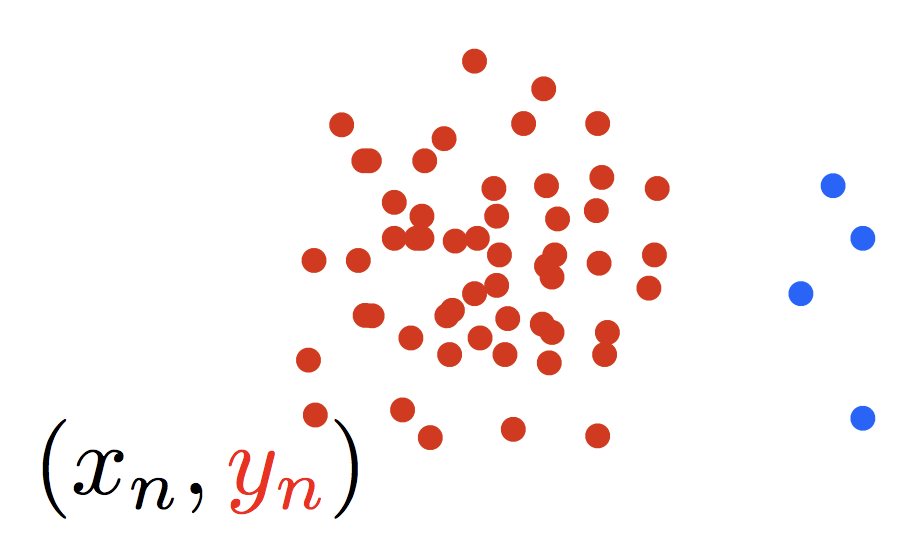
\includegraphics[width=0.5\textwidth]{binary}
\end{figure}

Intuitively, the blue points in the above figure is more ``important" than the red points, and should be sampled with higher probabilities. In fact, the key of the importance sampling method is how to characterize the ``importance" of each training example, and is often highly non-trivial.
\subsection{Importance Scores Based on Structural Information} 
We propose to characterize the importance of each point by looking at its structural information. It is widely assumed that (high-dimensional) data points in the training set are approximately from a low-dimensional manifold. To explore this property, some type of graphs are constructed whose nodes are the data points, e.g. kNN graphs, which can be viewed as a discretization of the manifold. 
\begin{figure}[h]
	%	\caption{Example of a parametric plot ($\sin (x), \cos(x), x$)}
	\centering
	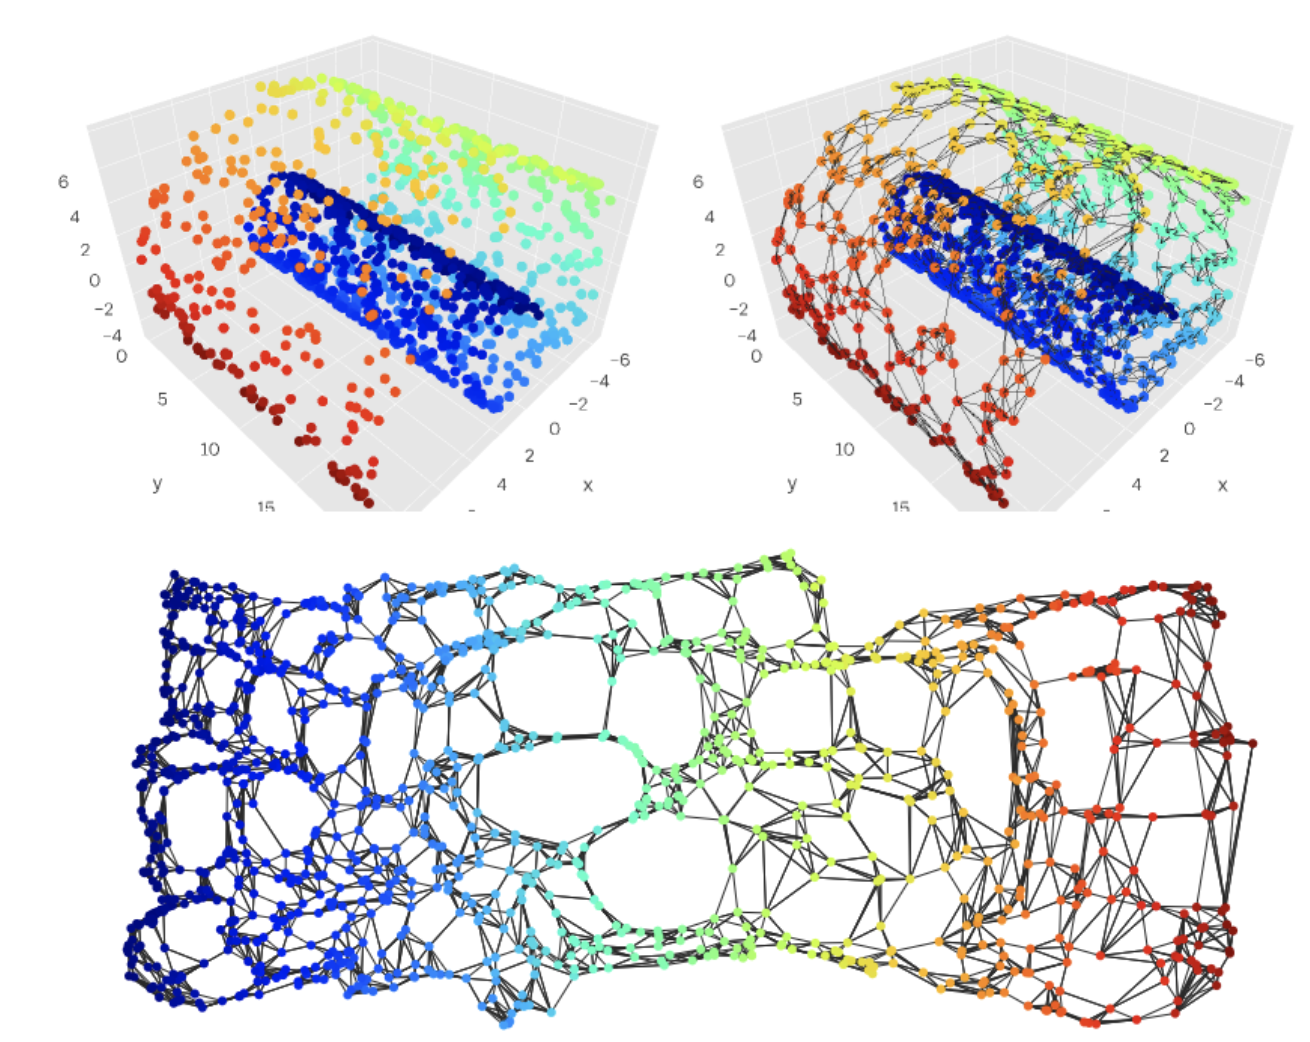
\includegraphics[width=0.5\textwidth]{manifold}
\end{figure}

Then, one can apply graph-based method (e.g., spectral clustering) for solving learning tasks. For our purpose, after the graph is constructed, we characterize the importance of each point, i.e., each node on the graph, using graph-theoretical tools, e.g., pagerank, random walk, centrality, diffusion, etc. Moreover, we can apply \emph{Graph Neural Networks} to automatically learn the importance of each node. 

\subsection{Model-dependent Importance Scores}
To learn the importance, the above method only consider data distribution information. However, the importance of the same point in the data set could be very different for different models. Thus, it could be of great help to utilize the properties of the model being trained to design model-dependent importance scores. For example, we could use Influence Functions, a classic tool from statistics, to characterize the importance of each point with respect to the model. It is also helpful to use a small proxy model to perform data selection, e.g., by removing hidden layers from the target model, using smaller architectures, and training for fewer epochs. Although these small proxy models have higher error rates, they could provide useful signals for coreset construction.

\subsection{Active Data Selection}
In the above methods, importance scores of all points and the subsample $\D'$ are determined in the beginning. Given $\D'$, we then train the model with stochastic mini-batch gradient methods. However, as the training process goes on, the inherent importance of each point may change. So, it is natural to assign importance scores in an adaptive manner. More precisely, we may sample the next mini-batch of data based on the current importance scores.  For this purpose, we can explore ideas from \emph{active learning}.
Conventional active learning selects points to label from a large pool of unlabeled data by repeatedly training a model on a small pool of labeled data and selecting additional examples to label based on the model’s uncertainty (e.g., the entropy of predicted class probabilities) or other heuristics. 

\section{Plan}
Since model-dependent methods are more complicated and it is much harder to make them work in practice, we mainly focus on model independent methods and the use of graph techniques. Coresets are widely studied for simpler problems such as $k$-means, logistic regression, Bayesian inference  etc., however, there is currently not much related work on general deep learning models. So, in the next stage, we need to implement and test some baseline methods for common data sets, eg. MINIST, CIFAR10, CIFAR100, ImageNet, and then extend these baseline to more sophisticated and effective approaches. The following two main challenges needs to be addressed: 1) how to exploit the properties the data manifold and what is the right way to build the underlying graph; 2) once the graph is built, which methods should be used to learn the importance scores for each node/example. We've been doing research on graph-based learning methods in recent years, and believe  such techniques will be of great help for our tasks. Next, we'll move to more realistic data sets and applications from Tencent. Finally, we will explore model-dependent and active learning methods.
 

%\bibliography{paper}
%\bibliographystyle{abbrv}
%\bibliographystyle{alpha}
\bibliographystyle{apalike}
\end{document}

